\section{Derivation of Moment Equations and their Approximation}

\begin{frame}{Shear Flow}
	\scriptsize
	\begin{align*}
		\partial_t f+ \nabla_{\boldsymbol{x}} \cdot(\boldsymbol{u} f) -\textcolor{red}{\nabla_{\boldsymbol{x}} \cdot\left((I+\boldsymbol{n} \otimes \boldsymbol{n}) e_3 f\right)}  &= -\textcolor{blue}{\nabla_{\boldsymbol{n}} \cdot\left(P_{\boldsymbol{n}^{\perp}} \nabla_{\boldsymbol{x}} \boldsymbol{u} \boldsymbol{n} f\right)} + \textcolor{blue}{D_r \Delta_n f}\label{SmochEq_kurz}, \\
		\operatorname{Re}\left(\partial_t \boldsymbol{u}+\left(\boldsymbol{u} \cdot \nabla_{\boldsymbol{x}}\right) \boldsymbol{u}\right) & =\Delta_{\boldsymbol{x}} \boldsymbol{u}-\nabla_{\boldsymbol{x}} p-\delta \left(\int_{S^{d-1}} f d \boldsymbol{n} \right) \boldsymbol{e_3} \\
		\nabla_{\boldsymbol{x}} \cdot \boldsymbol{u} & =0.
	\end{align*}
	Consider \textit{Shear Flow}, i.e. assume $	\boldsymbol{u} = (0,0,w(x,t))^T$, $f=f(x,t,\phi,\theta)$. \\
	\vspace{3mm}
	\pause
	In spherical coordinates and for the given velocity field $\boldsymbol{u}$, we get
	\begin{equation}
		\begin{aligned}
			\sin\theta \partial_{t}f & + \nabla_{\boldsymbol{x}} \cdot(\boldsymbol{u} f) + \textcolor{red}{\partial_x (\cos\phi \cos\theta \sin^2\theta f)} \\
			&= - \textcolor{blue}{\partial_\theta \left(w_x \sin^3 \theta \cos \phi f\right)} + \textcolor{blue}{D_{r} \left( \partial_\phi \left(\frac{1}{\sin \theta} \partial_\phi f \right) + \partial_\theta (\sin \theta \partial_\theta f) \right)}, \\
			& Re \partial_{t}w(x,t) = \partial_{xx}w + \delta \left( \bar{\rho} - \int_{0}^{2\pi} \int_{0}^{\pi} f \sin \theta \, d\theta \, d\phi \right). \label{SmochEq_wx}
		\end{aligned}
	\end{equation}
\end{frame}

\begin{frame}{Derivation of Moment Equations}
	\scriptsize
	Consider approximation of the form
	\begin{align}
		\textcolor{cyan}{f(\textbf{x}, t, \phi, \theta) \approx f^N(\textbf{x},t,\phi,\theta) :=  \sum_{n=0}^{N} \sum_{i=-2n}^{2n} c^i_{2n}(\textbf{x},t) \cdot P^i_{2n}(\phi, \theta)}, \label{spectralmethod}
	\end{align}
	where $P^i_{2n}(\phi, \theta)$, $n = 0, \ldots, N$, $i = -2n, \ldots, 2n$
 are harmonic polynomial basis functions, i.e., the eigenfunctions of the Laplace-Beltrami operator with the eigenvalue $-2n(2n+1)$. 
 \pause
 	\begin{itemize}
 	\item Insert ansatz $f^N =  \sum_{n=0}^{N} \sum_{i=-2n}^{2n} c^i_{2n}(x,t) \cdot P^i_{2n}(\phi, \theta)$ into kinetic equation
 	\begin{align*}
 		\sin\theta \partial_{t}f^N(x,t,\phi,\theta) + &  \textcolor{red}{\partial_x (\cos\phi \cos\theta \sin^2\theta f^N)} \\
 		& 
 		=- \textcolor{blue}{\partial_\theta \left(w_x \sin^3 \theta \cos \phi f^N\right)} +\textcolor{blue}{D_{r} \left( \partial_\phi \left(\frac{1}{\sin \theta} \partial_\phi f^N \right) + \partial_\theta (\sin \theta \partial_\theta f^N) \right)}
 	\end{align*}
 	\item Projection to the basis functions
 \end{itemize}
\end{frame}



\begin{frame}
	\scriptsize
	The system of moment equations has the general form
	\begin{align}
		\partial_t Q + \textcolor{red}{A\partial_x Q} = \textcolor{blue}{D(w_x)Q}+ \textcolor{blue}{D_rE Q},
	\end{align}
	where $Q=(c^0_0(x,t), c^{-2}_2(x,t), \ldots, c^{2N}_{2N}(x,t))^T$ represents the vector of the moments and \\
	\vspace{2mm}
	$A,D,E \in \mathbb{R}^{(N+1)(2N+1)x(N+1)(2N+1)}$.
	For $N=1$ the matrix $A$ has the form
	\begin{figure}[H]
		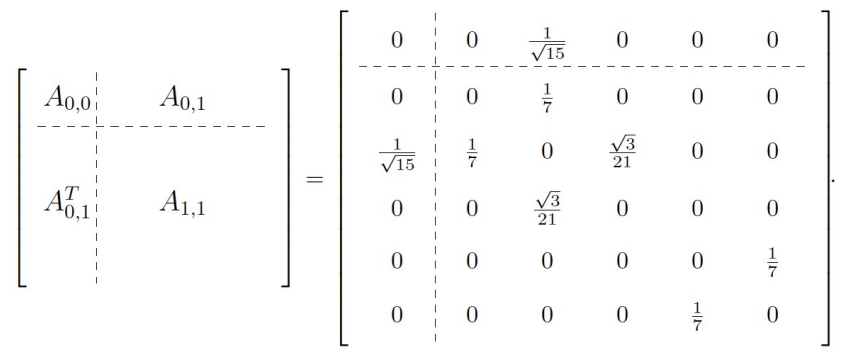
\includegraphics[scale=0.5]{Bilder/MatrixA}
	\end{figure}
\end{frame}


%----------------------------------------------------------
%----------------------------------------------------------

\begin{frame}{Rectilinear Flow}
	\scriptsize
	We consider $\boldsymbol{u} = \left( 0, 0, w(x,y, t)\right)^T$, $f(x,y,t,\phi,\theta)$. We get
	\begin{equation}
		\begin{aligned}
			&\sin\theta \partial_{t}f(x,y,t,\phi, \theta)+ \textcolor{red}{\partial_x(\cos\phi \sin\theta \cos\theta f)} + \textcolor{red}{\partial_y(\sin \phi \sin \theta \cos \theta f)} \\
			&+ \textcolor{blue}{\partial_\theta\left(( w_x \sin^3 \theta \cos \phi + w_y\sin \phi \sin^3 \theta) f\right)}
			= \textcolor{blue}{D_{r}\left( \partial_\phi \left(\frac{1}{\sin \theta} \partial_\phi f \right)+ \partial_\theta (\sin \theta \partial_\theta f)\right)} \\
			&Re\partial_{t}w(x,y,t) = \partial_{xx}w + \partial_{yy}w + \delta\left(\bar{\rho}-\int_{0}^{2\pi} \int_{0}^{\pi} f \sin \theta d\theta d\phi \right).
		\end{aligned}
	\end{equation}
	\pause
	The moment equations have the general form
	\begin{equation}
		\partial_t Q + \textcolor{red}{A  \partial_x Q}
		+ \textcolor{red}{B \partial_y Q} =  \textcolor{blue}{ D(w_x,w_y)Q+ D_rEQ}.
	\end{equation}
For $N=1$:
	\vspace{5pt}
\[
\scriptsize
\renewcommand{\arraystretch}{1.5} 
B =
\left[
\begin{array}{c:ccccc}  % ':' nach der ersten Spalte für vertikale gestrichelte Linie
	0 & 0 & 0 & 0 & \frac{\sqrt{15}}{15} & 0 \\
	\hdashline               % horizontale gestrichelte Linie nach der ersten Zeile
	0 & 0 & 0 & 0 & -\frac{1}{7} & 0 \\
	0 & 0 & 0 & 0 & 0 & \frac{1}{7} \\
	0 & 0 & 0 & 0 & \frac{\sqrt{3}}{21} & 0 \\
	\frac{\sqrt{15}}{15} & -\frac{1}{7} & 0 & \frac{\sqrt{3}}{21} & 0 & 0\\
	0 & 0 & \frac{1}{7} & 0 & 0 & 0
\end{array}
\right].
\]
\end{frame}

%----------------------------------------------------------
%----------------------------------------------------------

\begin{frame}{Coupled System for a Three-Dimensional Flow}
	\scriptsize
	We consider $\boldsymbol{u} = \left( 0, 0, w(x,y,z,t)\right)^T$, $f(x,y,t,\phi,\theta)$. We get
	\begin{equation}
		\begin{aligned}
			&\sin\theta \partial_{t}f(x,y,t,\phi, \theta)+ \textcolor{red}{\partial_x(\cos\phi \sin\theta \cos\theta f)} + \textcolor{red}{\partial_y(\sin \phi \sin \theta \cos \theta f)} - \textcolor{red}{\partial_z((1+ \cos^2 \theta)f)} \\
			&= -  \textcolor{blue}{\partial_\theta\left(( w_x \sin^3 \theta \cos \phi + w_y\sin \phi \sin^3 \theta - w_z \cos \theta \sin^2 \theta) f\right)} \textcolor{blue}{D_{r}\left( \partial_\phi \left(\frac{1}{\sin \theta} \partial_\phi f \right)+ \partial_\theta (\sin \theta \partial_\theta f)\right)} \\
			&Re\partial_{t}w(x,y,t) = \partial_{xx}w + \partial_{yy}w + \partial_{yy}z + \delta\left(\bar{\rho}-\int_{0}^{2\pi} \int_{0}^{\pi} f \sin \theta d\theta d\phi \right).
		\end{aligned}
	\end{equation}
	\pause
	The moment equations have the general form
	\begin{equation}
		\partial_t Q + \textcolor{red}{A  \partial_x Q}
		+ \textcolor{red}{B \partial_y Q} +  \textcolor{red}{C \partial_z Q} =  \textcolor{blue}{ D(w_x,w_y, w_z)Q+ D_rEQ}.
	\end{equation}
For $N=1$:
\[
\scriptsize
\renewcommand{\arraystretch}{1.5} 
C = \left[
\begin{array}{c:ccccc}
	-\frac{4}{3} & 0 & 0 & -\frac{2\sqrt{5}}{15} & 0 & 0 \\
	\hdashline        
	0 & -\frac{8}{7} & 0 & 0 & 0 & 0 \\
	0 & 0 & -\frac{10}{7} & 0 & 0 & 0 \\
	-\frac{2\sqrt{5}}{15} & 0 & 0 & -\frac{32}{21} & 0 & 0 \\
	0 & 0 & 0 & 0 & -\frac{10}{7} & 0\\
	0 & 0 & 0 & 0 & 0 & -\frac{8}{7}
\end{array}
\right].
\]
\end{frame}








